\documentclass{llncs}
\usepackage{graphicx,float,wrapfig}
\usepackage{epstopdf}
%
%\title{Experimental Platform for Human Robot Interaction based on Human Motions}
\title{An Intuitive Interface for designing Social behaviors based on Human motions}
%
\titlerunning{ExPhriMot}  % abbreviated title (for running head)
%                                     also used for the TOC unless
%                                     \toctitle is used
%
\author{Praveenkumar Vasudevan\inst{1} \and Gentiane Venture\inst{2}}
%
\authorrunning{Praveenkumar Vasudevan et al.} % abbreviated author list (for running head)
%
%%%% list of authors for the TOC (use if author list has to be modified)
\tocauthor{Praveenkumar Vasudevan, Gentiane Venture}
%
\institute{Graduate Student, \'{E}cole Centrale de Nantes, Nantes, France,\\
\email{praveenv4k@gmail.com}
\and
Associate Professor, Tokyo University of Agriculture and Technology, Japan\\
\email{venture@cc.tuat.ac.jp}}
\begin{document}

\maketitle   
\begin{abstract}
	Humans interacting with intelligent robots has been seen as a potential game changer of the future. In scenarios where robots coexist with humans in a social environment, understanding not only verbal communication, but also non-verbal communication is extremely inevitable. The non-verbal communication carries information such as intention, emotion and health of a human, that adds value to the way robots participate in an interaction. Additionally, the people who design interaction scenarios are from diverse fields who do not essentially have the required robot programming skills. In this paper we propose an easy to use and intuitive programming interface which gives the power to design robot behaviors taking into account human motions. We propose a distributed architecture which gives the capability to plug and play multi-modal motion recognition systems and diverse class of robots. We present results of Nao humanoid robot performing actions understanding human motions using kinect motion recognition system.
\keywords{human robot interaction, motion recognition, robot behaviors, kinect, nao}
\end{abstract}
%
\section{Introduction}
%
%Human-Robot interaction (HRI) has emerged as the most promising fields in the recent years owing to its immense potential in the fields of education, entertainment, elderly care and rehabilitation. 
\emph{Human Robot Interaction (HRI) is a challenging research field at the intersection of psychology, cognitive science, social sciences, artificial intelligence, computer science, robotics, engineering and human-computer interaction}\cite{Dautenhahn2007}. Goodrich\cite{Goodrich:2007:HIS:1348099.1348100} in his extensive survey proposed two main types of HRI namely Remote interaction or Teleoperation and Proximate interaction. The latter is particularly important where the humans and the robots are co-located (for example, service robots may be in the same room as humans). Proximate interaction has gained importance due to the successful encounters of putting robots to work with human beings. It has led to the development of a new class of robots called Social Robots. Fong et al. \cite{Fong2003} define that social robots are able to recognize each other and engage in social interactions; Breazeal et al.\cite{Breazeal:2002:DSR:515422} explain that a social robot is a robot which is able to communicate with humans in a personal way; Bartneck and Forlizzi \cite{Bartneck2004} describe that a social robot is an autonomous or semi-autonomous robot that interacts with humans by following some social behaviors; Hegel et al. \cite{Hegel2009} define that a social robot is a combination of a robot and a social interface. Summarizing all these Yan et al. \cite{Yan2014} defines \emph{“A social robot is a robot which can execute designated tasks and the necessary condition turning a robot into a social robot is the ability to interact with humans by adhering to certain social cues and rules.”}

The Social robots already entered the human spaces as entertainers\cite{NaoTheRobot}, educators\cite{NaoTheRobot}, caring agents\cite{ASKNao} and personal assistants\cite{ProjectRomeo}. Given that social robotics has emerged as a promising field, design and development of interaction systems need to be approached in a systematic manner wherein the robots should be able to understand the human motions and intentions in order to interact in a better way. To make it possible it is necessary to develop robotic systems with essential cognitive skills for efficient and natural interaction. Most often the on-board sensors on the robots fail to satisfy this demanding requirement due to various constraints like space, power and computational requirements. Hence consideration of augmenting exteroceptive sensors that are commonly available in the smart home/public environments to this purpose is important.

%However when it comes to designing complex behaviors, traditional flow chart based approaches[2] increase the cognitive load on the end users.
Another important aspect in HRI is the fact that the users of such systems are from diverse backgrounds. So the tools needed to design behaviors of a social robot should be intuitive and user friendly.  With increased availability of social robots and cost effective motion recognition sensors, we could observe a huge void which inhibits the exploitation of available technology for designing human motion driven robot behaviors. More efficient tools are needed which could tackle this issue.

The main contribution of this work will be to develop an application independent experimental platform wherein a social robot will be augmented with essential perceptual ability to understand human motions. The behavior design of such a social robot will be made possible by an easy to use behavior design interface. The resulting experimental platform could be used by people from interdisciplinary fields to design, evaluate and study specific aspects of the interaction between the social robot and the human.
%
%The key problem statements of this work are
%\begin{itemize}
%\item Human Pose estimation and motion recognition
%\item Localization of the robot
%\item Behavior design interface
%\end{itemize}
%
\section{Related work}
%
%\subsection{Human Pose Detection}
%
	Vision based motion capture and analysis has been studied widely and a summary of all the approaches developed during the past three decades have been presented in the surveys \cite{Moeslund2001231} \cite{Moeslund200690}\cite{Poppe20074}. Vision based human pose estimation has traditionally suffered from the requirement to adopt an initialization pose and losing track after a few frames. These problems have been addressed by the approaches by Xbox\cite{Kinect2014} team which are capable of accurately predicting the 3D positions of body joints using single depth images without using any temporal information\cite{Shotton2011}\cite{Shotton2013}. Unlike the approaches used in the Kinect SDK, the approach presented in \cite{Buys201439} uses both the depth and color(RGB-D) data for human body detection and pose estimation using a customizable human kinematic model. Understanding of human motion is not complete if the action of the human could not be understood. In the survey by Microsoft research\cite{KinectCV2013}, a background study on various algorithms used for human activity analysis is presented. Recently data-driven machine learning approaches like neural networks, Support vector machines, clustering, decision trees and bayesian networks have proven to be successful with recognition accuracy as high as 94\%\cite{KinectSDK2014}.\\
	The localization of humanoid robots is a challenging issue, due to rough odometry estimation, noisy onboard sensing, and the swaying motion caused by walking\cite{Cervera2012}. The Point cloud library\cite{RusuPCL11} which is one of the most widely used 3D perception software library, implements ready to use probabilistic tracking algorithms\cite{RUeda2012}. Studies on robot localization, obstacle mapping, and path planning in multilevel 3D environments by equipping Nao with a consumer-level depth camera has been reported in \cite{Maier2012}. Localization and motion planning in smart home environment using an external Kinect sensor have been proposed in \cite{Cervera2012}. In \cite{choi13_rgb_d_objec_track} a robust particle filter parallelized on a GPU that can track a known 3D object model over a sequence of RGB-D images is proposed. However all these methods are computationally demanding and it could cause overall performance degradation particularly when we want to share the same sensor for both motion recognition and localization of the robot.  Tracking rectangular fiducial markers using  augmented reality toolkits like ARToolKit\cite{Kato1999} can be interesting if we could embed those markers on the humanoid robot. This is one of the simplest and cheapest solution in terms of the computational power as it can provide position and orientation of the physical markers in real time.\\
	The users of social robots do not have necessary backgrounds in programming and design of robot behaviors. The main challenge in the behavior design is the ability to define the behavior which can abstract complex data flows from the end user. There exists several flow-chart based visual programming languages\cite{MSRS4},\cite{Choregraphe} which allow non-programmers to create robot applications using a set of pre-built behavioral blocks. These programs are very intuitive and allow the users to realize complex sequence of movements and sequential behaviors. However when it comes to designing reactive behaviors for human-in-the-loop scenarios, the existing visual programming methods increase the cognitive load on the end users. Specialized robot programming techniques like Task description language\cite{Simmons724883}, scripting techniques like Universal Robotic Body Interface(URBI)\cite{Baillie4814281} and ROS\cite{quigley2009ros} have been proposed in the literature. Though these programs provide modularity, distributed nature ,support multiple sensors and robots, all these tools require high level of skill in robotics and programming skill to use them. Recently a new non-domain-specific solution called \emph{Target Drives Means} is proposed in \cite{BerenzTDM2014} however it lacks an intuitive interface.
	Recently there has been lot of efforts to teach programming to children and people without computer science background\cite{Scratch}\cite{TouchDevelop}\cite{Blockly}. These tools are very intuitive and have already been proven to be used by novice programmers to build games and educational applications. The Blockly library\cite{Blockly} from Google offers a complete client side javascript library which could be used for developing custom blocks and code generators as per the application requirements.
%Hierarchical organization of behaviors and modularity are also being investigated \cite{Jaegeretal},\cite{Baldassarre:2013:CRM:2560111},\cite{hurdus4648045}
%\subsection{Behavior Design Frameworks}
\section{Motion Driven Behavior Interface}
%
We propose a light weight interface for designing human motion driven behaviors taking inspiration from distributed architecture like ROS\cite{quigley2009ros} and intuitive visual programming techniques. 
%
\subsection{System Architecture}
%
The important components of the system are
\begin{itemize}
\item Application Components
\begin{itemize}
\item Context: The application context contains the complete description of the world. It contains latest information about the robots and humans in the environment
\item Parameter Server: The parameter server acts as a central repository for managing the parameters of distributed components and the system.
\item Embedded Web Server: The web server embedded in the application serves the data requests from the client
\item Context Orchestrator: The orchestrator collect uptodate information about the robot and human in the environment and updates the Context.
\item Bootstrapper : The bootstrapper takes care of initializing the system and starting up all the pre-configured nodes. It also takes of starting and stopping the behavior programs when requested by the user.
\end{itemize}
\item Distributed Components : These are nodes in the system each with a specific goal that can be started/stopped at any time during the entire application life-cycle without affecting the other nodes or the system. All the nodes will communicate with the application using message passing techniques.
\begin{itemize}
\item Motion Recognition Node : A dedicated node that interacts with a motion recognition sensor and sends the detected gestures and motions to the application. Additionally each motion recognition module registers a set of actions/gestures that could be detected with the sensor associated with it.
\item Robot Interface Node : A dedicated node that interacts with a specific robot and can invoke a set of actions on it. It also sends periodic update about the Robot status to the application. Moreover it registers a set of actions that could be invoked on the robot associated with it.
\item Behavior Program Node : A dynamic node that will be created when the user starts the program he/she designed using the user interface. The declarative description of the behavior is parsed in order to create a memory mode The Behavior program node monitors the action triggers and invokes the corresponding robot actions according to the way it is being described in the program.
\end{itemize}
\item User Interface: The user interface is a web application that runs on any latest webkit browsers supporting WebGL. 
\begin{itemize}
\item Behavior Designer: The Behavior designer surface could be used by the user to drag and drop the behavior blocks and construct the program using the set of motion capabilities registered by the active motion recognition nodes and the set of robot action capabilities registered by the active robot interface nodes. The behavior described using the designer will be encoded into a declarative XML format and sent to the server when the user request to start the program
\item Visualization: The visualization could be used to see the interaction of the human and robot inside a 3D environment.
\end{itemize}
\end{itemize}
\begin{figure}
\centering
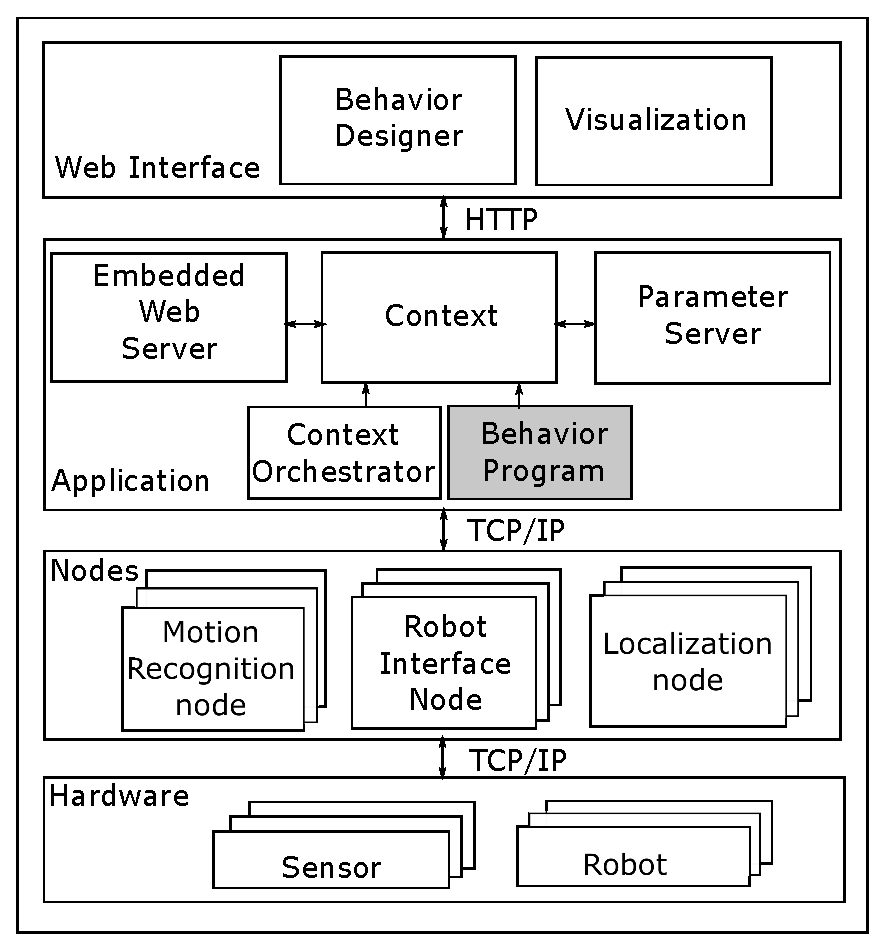
\includegraphics[width=1\textwidth]{../thesis/assets/architecture.eps}
\caption[System Architecture]{System Architecture}
\label{fig:architecture}
\end{figure}
%
\subsection{Implementation}
%
%
\section{Experimentation}
%
%
\section{Conclusions}
%
For the moment we have evaluated our system only for the Kinect motion capture system working seamlessly with the Nao humanoid robot for a set of predefined gestures and robot actions. We are planning to develop an extensive database containing commonly encountered gestures and also an extensive set of primitive robot actions. These will be made available to the end user through the intuitive programming interface which could be then used for defining complex motion driven behaviors. Additionally we are also planning to integrate our system to work with other modes of motion recognition like IMU, Accelerometers and Gyroscopes that are available in smart-phones and wearable devices. Similarly we would like to integrate other system with other robots like Pepper which we expect to receive soon.
%
\section{Acknowlegdements}
%
		We would like to thank the members of GVLab of Tokyo University of Agriculture and Technology for helping us arranging the resources to realize this work and participate in the experimentation.
%
% ---- Bibliography ----
%
%\begin{thebibliography}{5}
%
\bibliographystyle{plain}
\bibliography{Bibliography}
%\bibitem {clar:eke}
%Clarke, F., Ekeland, I.:
%Nonlinear oscillations and
%boundary-value problems for Hamiltonian systems.
%Arch. Rat. Mech. Anal. 78, 315--333 (1982)
%
%\bibitem {clar:eke:2}
%Clarke, F., Ekeland, I.:
%Solutions p\'{e}riodiques, du
%p\'{e}riode donn\'{e}e, des \'{e}quations hamiltoniennes.
%Note CRAS Paris 287, 1013--1015 (1978)
%
%\bibitem {mich:tar}
%Michalek, R., Tarantello, G.:
%Subharmonic solutions with prescribed minimal
%period for nonautonomous Hamiltonian systems.
%J. Diff. Eq. 72, 28--55 (1988)
%
%\bibitem {tar}
%Tarantello, G.:
%Subharmonic solutions for Hamiltonian
%systems via a $\bbbz_{p}$ pseudoindex theory.
%Annali di Matematica Pura (to appear)
%
%\bibitem {rab}
%Rabinowitz, P.:
%On subharmonic solutions of a Hamiltonian system.
%Comm. Pure Appl. Math. 33, 609--633 (1980)

%\end{thebibliography}
\end{document}